\chapter{Choosing light sources and modulation}
\label{ch:lasers}

Do not choose a laser by comparing data sheets in isolation. Start with reach,
lane rate, fiber plant, power, cost, lifetime, manufacturing volume, and service
policy. Those requirements select an architecture. The architecture then limits
the useful source, modulation, detector, packaging, and validation choices.

\section{System requirements and architecture paths}
\label{sec:laser-system-requirements}

Freeze the system problem before asking a supplier for samples:

\begin{dectree}
Reach / fiber plant
  |
Lane rate / bandwidth
  |
Laser choice
  |
Modulator path
  |
Receiver / detector
  |
Validation burden (ATP, lock, thermal, life)
\end{dectree}

\begin{description}
\item[Reach and fiber] decide whether multimode loss and modal bandwidth are
      acceptable or whether the link needs single-mode fiber.
\item[Lane rate and bandwidth] decide whether direct modulation closes the eye or
      whether the link needs an EML, MZM, or ring.
\item[Power and cooling] include laser wall-plug power, modulator loss, driver
      power, TEC power, and control overhead.
\item[Cost and volume] include fiber plant, assembly alignment, burn-in, test time,
      yield, and field replacement, not only die price.
\item[Reliability and service] decide whether the source can stay inside the
      package or must be a replaceable ELSFP.
\end{description}

The choices are coupled. A cost-driven, short multimode link points toward an
850~nm VCSEL, multimode fiber, silicon photodiodes, and direct modulation. A
longer single-mode path points toward a 1310~nm DFB or EML and germanium or
III-V detection. Dense WDM and co-packaged optics often move the CW source away
from the modulator, which adds wavelength control, fiber attach, and service
requirements. \Cref{sec:laser-reqs,tab:laser-req-fork} turns these paths into
supplier specifications.

\section{Light-source and modulation choices}

The short-reach market uses a small set of source families. Each fits a different
constraint set:

\begin{description}
\item[DFB (distributed feedback)] a grating along the active region gives
      single-mode output; the workhorse continuous-wave (CW)\firstterm{CW} or directly
      modulated source for CWDM and LAN-WDM (\Cref{sec:dfb-eml}).
\item[DBR (distributed Bragg reflector)]\firstterm{DBR} the grating sits outside
      the gain region. Choose it when tunability or separate control of gain and
      wavelength is worth added control and qualification work.
\item[External-cavity laser] a gain element and an external wavelength-selective
      cavity provide narrow linewidth and tunability. Choose it when spectral
      purity or lock range matters more than package size, cost, and control-loop
      simplicity. Most short-reach IM/DD links do not need it
      \cite{eclplanex}; the cited product is vendor orientation, not a datacenter
      source recommendation.
\item[DML (directly modulated laser)]\firstterm{DML} modulate the bias current directly: cheap
      and low-power, but chirp-limited over dispersive fiber (\Cref{sec:dml-vcsel}).
\item[EML (externally modulated laser)] \term{EML}\firstterm{EML}: a DFB integrated with an
      \term{EAM}\firstterm{EAM}. Low chirp and high bandwidth make it
      the dominant 100--200G/lane transmitter for single-mode links at DR (500~m)
      and shorter (\Cref{sec:dfb-eml,sec:eml-eam}).
\item[CW laser + TFLN MZM] an external CW source feeds a thin-film lithium
      niobate Mach--Zehnder modulator on a separate chip. Very low chirp and
      $\gtrsim$100~GHz EO bandwidth make this the leading path to 400G/lane
      pluggables and high-baud FR links; see \Cref{sec:tfln-mzm,tab:tx-modulator}.
\item[CW laser + Si MZM] an external CW source feeds a silicon Mach--Zehnder
      modulator on the same PIC (\Cref{sec:simzm}). Low chirp, flat passband, and
      CMOS fab integration make this the default for 100--200G/lane DR/FR SiPh
      modules; 400G/lane demos appeared in 2026.
\item[CW laser + Si ring] same laser architecture, but a microring or microdisk
      modulator on the PIC (\Cref{sec:siring}). Smaller footprint and strong WDM/CPO
      fit; wavelength lock and thermal crosstalk dominate validation (\Cref{ch:wdm}).
\item[CW-WDM / multi-wavelength sources] high-power, multi-wavelength CW lasers
      (per the CW-WDM MSA) that feed comb-like WDM architectures
      (\Cref{sec:cwwdm-laser,sec:cwwdm}).
\item[VCSEL]\firstterm{VCSEL} 850--940~nm multimode sources for short-reach links over multimode
      fiber; cheap but reach-limited and less relevant at 200G/lane.
\item[External laser source (ELS/ELSFP)] a pluggable laser module supplying CW
      light to a co-packaged switch, so a failed laser is field-replaceable
      (\Cref{sec:elsfp}).
\end{description}

\begin{table*}[ht]
\refstepcounter{table}\label{tab:source-mod-matrix}%
\centering
\setlength{\tabcolsep}{2.5pt}%
\scriptsize
\renewcommand{\arraystretch}{1.25}%
\begin{tabular}{@{}p{0.12\linewidth}p{0.13\linewidth}p{0.13\linewidth}p{0.13\linewidth}p{0.13\linewidth}p{0.13\linewidth}p{0.13\linewidth}@{}}
\toprule
Attribute & VCSEL direct & DFB direct & DFB + EAM & CW DFB/DBR + MZM & CW DFB/DBR + ring & External cavity + modulator \\
\midrule
Wavelength / fiber & 850--940~nm / MMF & 1310~nm / SMF & 1310~nm / SMF & 1310 or 1550~nm / SMF & WDM grid / SMF & Tunable grid / SMF \\
\addlinespace[1.5em]
Modulation fit & Direct only & Direct & Integrated EML & Si or TFLN MZM & Resonant Si ring & External MZM or ring \\
\addlinespace[1.5em]
Bandwidth / reach & Short, modal limit & Chirp-limited & High BW, low chirp & High BW, broad passband & High BW, lock-limited & High BW, architecture-specific \\
\addlinespace[1.5em]
RIN / linewidth & RIN and modal noise & RIN and chirp & RIN plus EAM bias & RIN; linewidth usually secondary & RIN plus spectral alignment & Low linewidth; verify feedback response \\
\addlinespace[1.5em]
Power / efficiency & Low Tx complexity & Low Tx complexity & Driver and EAM loss & Laser, driver, and MZM loss & Laser, heater, and lock power & Laser plus control overhead \\
\addlinespace[1.5em]
Reliability & Junction and temperature wear & Facet and active-region wear & Laser plus EAM aging & Source, attach, and bias drift & Source, heater, and lock faults & Cavity, package, and lock faults \\
\addlinespace[1.5em]
Manufacturing & Array-friendly, MMF plant & Simple Tx, SMF attach & Mature integrated Tx & Multi-die attach and RF match & Dense PIC, tight thermal control & Tight optical assembly and control \\
\addlinespace[1.5em]
Validation burden & Modal, temperature, aging & Chirp, LIV, RIN & LIV, RIN, EAM sweep, TDECQ & Source plus bias and RF path & Source plus resonance and crosstalk & Spectrum, lock, feedback, environment \\
\bottomrule
\end{tabular}
\par\medskip
{\raggedright\footnotesize\textbf{Table~\thetable.} Decision matrix for common
source and modulation paths. Entries show the dominant engineering concern, not
fixed rankings. Program limits come from \Cref{tab:laser-prd}.\par}
\end{table*}
\FloatBarrier

\subsection{Reading the source and modulation matrix}
\label{sec:source-mod-matrix-read}

\Cref{tab:source-mod-matrix} is a decision map across paths, not a datasheet.
Read it by \emph{attribute row}: each row asks one engineering question that
every path must answer. Family detail for VCSEL, DML, EML, MZM, and rings
follows in later sections; use this matrix to see which questions become hard
before you commit.

\paragraph{Wavelength / fiber.}

\textbf{Purpose.}
Which wavelength band and fiber type does the path assume?

\textbf{Uncertainty removed.}
Reach, plant, and WDM grid are not free variables after this choice. MMF at
850--940~nm and SMF at 1310/1550~nm pull different connectors, modal limits,
and lock burdens.

\textbf{Decision unlocked.}
Accept the plant class, or reject a path that cannot meet the fiber and grid
requirement.

\textbf{Risk if skipped.}
You pick a modulator before you know whether the link is MMF short-reach or
SMF WDM.

\paragraph{Modulation fit.}

\textbf{Purpose.}
Is the path direct modulation, integrated EAM, external MZM, or resonant
ring?

\textbf{Uncertainty removed.}
Driver, chirp, and lock problems change with the modulator class. Direct
paths buy simplicity and pay chirp or modal limits; external paths buy
bandwidth and pay attach and control.

\textbf{Decision unlocked.}
Allocate driver, bias, and control ownership for the chosen modulator class.

\paragraph{Bandwidth / reach.}

\textbf{Purpose.}
Can the path close the baud and reach without a physics veto?

\textbf{Uncertainty removed.}
Modal bandwidth, chirp, or lock range may kill a path before cost discussions
matter.

\textbf{Decision unlocked.}
Keep the path, derate reach/rate, or move to a higher-BW class (for example
EML or MZM over DML).

\paragraph{RIN / linewidth.}

\textbf{Purpose.}
Which noise and spectral purity limits dominate the BER floor and WDM fit?

\textbf{Uncertainty removed.}
Isolator-free and reflection-rich plants harden RIN. Rings and WDM harden
spectral alignment. External cavities often win linewidth but still need
feedback checks.

\textbf{Decision unlocked.}
Set RIN@ORL and SMSR/linewidth requirements in \Cref{tab:laser-prd}.

\paragraph{Power / efficiency.}

\textbf{Purpose.}
Where does wall-plug and optical power go: laser only, or laser plus driver,
EAM/MZM loss, heaters, and lock?

\textbf{Uncertainty removed.}
``Efficient laser'' claims fail if heater and lock power dominate the module
budget.

\textbf{Decision unlocked.}
Accept the power split, or reject a dense path that breaks the rack power
envelope.

\paragraph{Reliability.}

\textbf{Purpose.}
Which wear-out and fault classes own life: junction, facet, EAM, attach,
heater, or lock?

\textbf{Uncertainty removed.}
Life models and FA paths differ by class (\Cref{sec:wearout-modes}). An
integrated source makes laser yield a package risk; an ELS makes the optical
interface a service risk.

\textbf{Decision unlocked.}
Name the life owner and the screens (HTOL, EAM age, mate cycles) before NPI.

\paragraph{Manufacturing.}

\textbf{Purpose.}
What assembly and plant skills does the path demand?

\textbf{Uncertainty removed.}
Array MMF plants, SMF attach, multi-die RF match, and dense PIC thermal
control are different factories. Path choice is also a supplier-capability
choice.

\textbf{Decision unlocked.}
Pick a path the supply chain can screen, or fund the missing process.

\paragraph{Validation burden.}

\textbf{Purpose.}
Which measurements become mandatory because of the path?

\textbf{Uncertainty removed.}
VCSEL needs modal and temperature work. EML needs LIV, RIN, EAM sweep, and
TDECQ. Rings need resonance, crosstalk, and lock. External cavities need
spectrum, lock, and feedback.

\textbf{Decision unlocked.}
Size the ATP and DVT matrix to the path; do not copy another product's
checklist blindly.

\subsection{How to use the matrix}

\begin{enumerate}
\item Freeze wavelength/fiber and reach/rate from the product requirements.
\item Strike paths that fail bandwidth/reach or plant class.
\item Among survivors, score RIN/linewidth, power, reliability, and
      manufacturing against your constraints.
\item Read the validation-burden row as a cost: every hard cell is an ATP
      and FA investment you must fund.
\item Fill \Cref{tab:laser-prd} from the winning path; reject alternatives
      with a one-line reason retained for review.
\end{enumerate}

Later sections teach each family. Do not let family enthusiasm override a row
that already vetoes the path.

\subsection{Learning summary}

\begin{description}
\item[Wavelength / fiber] Plant and grid first.
\item[Modulation / BW] Physics veto before cost.
\item[RIN / power / reliability] The ledgers that usually decide.
\item[Manufacturing / validation] Can you build and screen it repeatedly?
\end{description}

\section{Directly modulated lasers and VCSELs}
\label{sec:dml-vcsel}

Before EMLs and silicon photonics took over single-mode datacenter ports, most
volume optics were either a cheap \term{DML} on single-mode fiber or a
\term{VCSEL} array into multimode fiber. Both still matter at the low-cost,
short-reach edge of the market, and both show why chirp, modal bandwidth, and
temperature push AI fabrics toward externally modulated single-mode sources.

A DML modulates laser bias current directly. The transmitter is simple and
efficient, but the same carrier dynamics that make modulation easy also produce
chirp: intensity changes drag the optical frequency along
(\Cref{sec:chirp-dispersion}). Over multimode or very short single-mode runs that
is often acceptable. Over dispersive single-mode fiber at tens of GBd, the chirp
turns into inter-symbol interference and closes the eye. Validation therefore
focuses on extinction ratio, pattern-dependent chirp, and RIN, not just average
power.

VCSELs took a different path. They emit from a vertical cavity at 850--940~nm
straight into multimode fiber, so parallel arrays are easy to assemble and cheap
to ship. That combination made VCSEL SR optics the default for early 40G/100G
Ethernet inside the rack (100G-SR4 and its cousins): short ribbons of MMF, high
lane count, low dollars per gigabit. The same physics that made them attractive
also capped their future. Multimode fiber has modal bandwidth and modal noise
limits; VCSEL bandwidth and reliability both degrade with temperature; and as
lane rates climb toward 100~G and 200~G, those limits arrive sooner. The industry
response has been incremental (better OM4/OM5 fiber, tighter specs, sometimes
PAM4 on MMF) rather than a clean leap to 400G/lane SMF DR. In practice, MMF
reach and modal dispersion keep VCSEL links in the SR box
(\Cref{sec:pmd-reach}), while hyperscale AI fabrics standardize on single-mode
DR/FR and CPO.

Neither family is the path to 400G/lane SMF DR. EMLs and external modulators
(\Cref{sec:dfb-eml,sec:simzm,tab:tx-modulator}) own that space. Pattern-aware
chirp linearization can stretch a DML a little farther, but it does not change
the physics at FR distances: if you need low chirp and high EO bandwidth at
fleet scale, you leave direct modulation behind.

\section{DFB and EML: the workhorse transmitters}
\label{sec:dfb-eml}

Once single-mode DR/FR became the hyperscale default, most short-reach ports
started with an InP\firstterm{InP} laser chip. Two configurations still dominate production:
the CW or directly modulated DFB, and the EML that adds an electro-absorption
modulator on the same die.

\paragraph{DFB.} A distributed-feedback laser has a grating along the active region
that selects one longitudinal mode. Spec-sheet metrics that matter in bring-up are
threshold current, slope efficiency, SMSR (typically many tens of dB on a clean
part), RIN, and wavelength vs.\ temperature/current. Used as a CW source for SiPh
or TFLN modulators, or as a DML when chirp is acceptable (\Cref{sec:dml-vcsel}).
Uncooled datacom DFBs ride case temperature with a known $d\lambda/dT$; cooled
parts add a TEC\firstterm{TEC} and lock to a grid.

\paragraph{EML.} An electro-absorption modulated laser integrates a DFB with an
\term{EAM} on one chip (\Cref{sec:eml-eam}). Reverse bias on the EAM sets absorption
and extinction; chirp stays far below a DML. That combination, not marketing, is
why EMLs became the volume answer for 100G/lane and then 200G/lane DR/FR
pluggables: one chip, low chirp, mature supply chain. Validation adds EAM bias
sweeps, aging of the absorption curve, and driver-match checks on top of the DFB
LIV/SMSR/RIN suite (\Cref{sec:laser-params,sec:laser-aging}).

\paragraph{When to pick which.} Through 200G/lane DR, EML usually wins on cost and
integration. A CW DFB (or ELSFP/CW-WDM bank) plus Si MZM, ring, or TFLN wins when
the modulator must sit on silicon or needs $\gtrsim$100~GHz EO bandwidth
(\Cref{tab:tx-modulator,sec:simzm,sec:siring,sec:tfln-mzm}). At CPO scale the laser
often leaves the optical engine entirely so it can be replaced without pulling the
ASIC package (\Cref{sec:elsfp}). Looking forward, 400G/lane pluggables are pushing
harder toward external CW plus TFLN or high-BW silicon modulators, while EMLs
remain the workhorse of the installed 100--200G base.

\begin{table*}[ht]
\refstepcounter{table}\label{tab:laser-choice}%
\centering
\setlength{\tabcolsep}{5pt}%
\renewcommand{\arraystretch}{1.25}%
\begin{tabular}{@{}p{0.14\linewidth}p{0.24\linewidth}p{0.58\linewidth}@{}}
\toprule
Source & Typical use & Top risks \\
\midrule
DML & short reach, cost-driven & chirp/dispersion, extinction ratio \\
\addlinespace[1.5em]
EML & $\le$DR, 100--200G/lane & EAM bias/aging, thermal \\
\addlinespace[1.5em]
CW + TFLN MZM & 400G/lane FR/DR, NPO & MZM bias drift, fiber attach, driver match \\
\addlinespace[1.5em]
CW + Si MZM & DR/FR SiPh, 100--400G/lane & driver match, bias drift, fiber coupling \\
\addlinespace[1.5em]
CW + Si ring & CPO, WDM transceivers & wavelength lock, thermal crosstalk, coupling \\
\addlinespace[1.5em]
VCSEL & SR over MMF & modal noise, reach, temperature \\
\addlinespace[1.5em]
ELS / ELSFP & co-packaged optics & connectorization, fleet serviceability \\
\bottomrule
\end{tabular}
\par\medskip
{\raggedright\footnotesize\textbf{Table~\thetable.} When each source is used, and its top validation risks.\par}
\end{table*}

Use \Cref{tab:laser-choice} as a short risk card once the path is roughly
known. Use \Cref{tab:source-mod-matrix} when you still need to compare
attribute rows across paths. Do not treat this card as a substitute for the
full matrix or for \Cref{tab:laser-prd}.

\section{Choosing the modulation path}
\label{sec:siph-platforms}

The source decision and modulation decision must close together. Direct
modulation minimizes parts and power but carries laser chirp into the link. An
EML adds an EAM on the laser die and is a mature low-chirp path for
100--200G/lane. A silicon MZM uses more area and drive but gives a broad optical
passband. A ring is compact and fits dense WDM, but adds resonance control and
thermal-crosstalk tests. TFLN offers high bandwidth and low chirp with a separate
material platform and assembly flow.

\Cref{tab:source-mod-matrix} compares the system consequences. The device
operation, bandwidth, insertion loss, and driver interfaces live in
\Cref{sec:eml-eam,sec:simzm,sec:siring,sec:tfln-mzm,tab:tx-modulator}. Keep that
physics in one place. Here the decision is whether the link can carry the added
power, control, assembly, and validation burden.

\section{Laser requirements: from roadmap to specs}
\label{sec:laser-reqs}

Laser requirements only work when they are numbers a supplier can fail and a link
budget can close. Start from the interconnect roadmap choice, then fill a short
requirements slice; the ATP in \Cref{sec:supplier-exec} is how that slice is
enforced on every lot.

\paragraph{Roadmap forks that set the laser.}
Each architecture decision forces a different requirements set
(\Cref{tab:laser-req-fork}):

\begin{table*}[ht]
\refstepcounter{table}\label{tab:laser-req-fork}%
\centering
\setlength{\tabcolsep}{3.5pt}%
\footnotesize
\renewcommand{\arraystretch}{1.25}%
\begin{tabular}{@{}p{0.22\linewidth}p{0.28\linewidth}p{0.44\linewidth}@{}}
\toprule
Roadmap choice & Laser implication & Specs you must freeze early \\
\midrule
Pluggable EML vs CW+Si/TFLN & Integrated EAM vs external CW + modulator & EAM bias/aging and TDECQ vs CW power class, RIN, and modulator $V_\pi$ match \\
\addlinespace[1.5em]
On-package laser vs ELSFP/CW-WDM & Field replace vs FIT inside the package & Connector/ORL/mate cycles and hot-swap CMIS vs COD/aging inside ASIC thermal \\
\addlinespace[1.5em]
Isolator vs isolator-free (CPO) & Feedback tolerance vs quiet RIN only & Stressed $\mathrm{RIN}_x\mathrm{OMA}$ at stated ORL; monitor PD / lock policy \\
\addlinespace[1.5em]
Single-$\lambda$ vs CW-WDM / comb & One line vs $N$ lines into rings/filters & Per-line power flatness, SMSR, grid, crosstalk (\Cref{sec:cwwdm-laser}) \\
\addlinespace[1.5em]
Retimed vs LPO & Module DSP hides Tx vs host sees raw eye & Laser+modulator TDECQ/RLM floor vs host COM budget (\Cref{sec:com,sec:drivers}) \\
\addlinespace[1.5em]
Derate policy & Operating $I$, $T$, power below abs-max & Bias window, thermal class, FIT/$E_a$ assumptions (\Cref{sec:laser-aging}) \\
\bottomrule
\end{tabular}
\par\medskip
{\raggedright\footnotesize\textbf{Table~\thetable.} Architecture forks and the laser
specs each one forces. Freeze these before DVT samples are built
(\Cref{sec:supplier-exec}).\par}
\end{table*}

Each ``Specs you must freeze early'' cell is the exit criterion for that fork.
\textbf{Exit when} every active fork has numbers (or explicit N/A) before DVT
samples are built.

\paragraph{One-page requirements slice.}
\Cref{tab:laser-prd} is the PRD-sized list. Fill every row with a number (or an
explicit ``N/A for this architecture'') before you negotiate ATP limits. Do not
leave RIN without an ORL, or power without a case-temperature class.

\begin{table*}[ht]
\refstepcounter{table}\label{tab:laser-prd}%
\centering
\setlength{\tabcolsep}{3pt}%
\footnotesize
\renewcommand{\arraystretch}{1.25}%
\begin{tabular}{@{}p{0.16\linewidth}p{0.22\linewidth}p{0.20\linewidth}p{0.18\linewidth}p{0.18\linewidth}@{}}
\toprule
Parameter & How to set the number & Measure / ATP & Reject if & Derate / ops note \\
\midrule
Launch power / class & Link budget + connector loss + aging margin (\Cref{sec:link-budget}) & Power meter; ELSFP class & Below min at rated $T$ & Cap max power for COD \\
\addlinespace[1.5em]
Wavelength / grid & PMD or ring FSR plan; $d\lambda/dT$ headroom (\Cref{ch:wdm}) & OSA / wavemeter & Off-grid at case $T$ & TEC setpoints \\
\addlinespace[1.5em]
SMSR floor & Datasheet + modal-noise budget & OSA & Below floor at $T$ & Watch aging \\
\addlinespace[1.5em]
RIN (quiet + stressed) & BER floor vs BW (\Cref{sec:rin}); ORL from plant & PD+ESA; stated ORL & Above limit at ORL & Bias-driver noise budget (\Cref{sec:laser-drivers}) \\
\addlinespace[1.5em]
Bias window & LIV kink-free range at max case $T$ & LIV & Kink in window & Run below abs-max $I$ \\
\addlinespace[1.5em]
EAM / MZM (if any) & ER, RLM, TDECQ at baud (\Cref{sec:tdecq}) & DCA + bias sweep & TDECQ/RLM fail & Bias aging policy \\
\addlinespace[1.5em]
ORL / isolator & Architecture: isolator-free needs tighter RIN & ORL meter; mate cycles & ORL out of range & Cleaning / ELS mate life \\
\addlinespace[1.5em]
CMIS monitors & What fleet triage will read (\Cref{sec:fleet-triage}) & CMIS dump & Missing alarms / bad state machine & Enable sequence (\Cref{sec:bringup}) \\
\addlinespace[1.5em]
FIT / life & Fleet failures/day target (\Cref{sec:fit-example}) & GR-468 + $E_a$ & Screen escape & Burn-in depth; ELS replace \\
\bottomrule
\end{tabular}
\par\medskip
{\raggedright\footnotesize\textbf{Table~\thetable.} Laser requirements one-pager. Every
cell needs a program number; this table is the structure, not the limits.\par}
\end{table*}

\paragraph{How to fill numbers (method, not invention).}
Work backward from the link, not forward from a marketing slide. The four steps
below turn an architecture choice into ATP limits:

\begin{enumerate}
\item Close the optical ledger at target pre-FEC BER
      (\Cref{sec:link-budget,sec:kp4}). That sets minimum launch OMA/power and
      maximum allowed penalties (transmitter and dispersion eye closure quaternary,
      TDECQ; ORL/RIN).
\item From receiver BW and the RIN ceiling $Q_{\max}=1/\sqrt{\mathrm{RIN}\cdot\mathrm{BW}}$
      (\Cref{sec:rin}), set a stressed RIN limit with margin under the plant ORL you
      will actually see (not only a quiet bench).
\item From case-temperature and derating policy, set the LIV bias window and
      thermal class so the laser never sits on a kink or at abs-max in the fleet
      (\Cref{sec:laser-aging,sec:prod-corners}).
\item From service model, choose ELSFP mate-cycle / hot-swap requirements or accept
      on-package FIT and write COD/aging screens accordingly (\Cref{sec:elsfp}).
\end{enumerate}

Hand the filled slice to the supplier with the ATP checklist
(\Cref{tab:atp-laser}). If a roadmap slide cannot point to a row in
\Cref{tab:laser-prd}, the requirement is not real yet.

\textbf{Exit when} every cell in \Cref{tab:laser-prd} is a program number or
explicit N/A, with ORL stated wherever RIN appears and case-$T$ class stated
wherever power or bias appears. \textbf{Decision unlocked:} negotiate ATP
limits, or reopen the architecture fork that left a cell empty.

\keyidea{Laser leadership is a requirements sheet: architecture forks force
specific specs (power, grid, RIN@ORL, SMSR, bias window, CMIS, FIT). Fill
\Cref{tab:laser-prd} from the link budget and fleet model, then enforce it with
the ATP (\Cref{sec:supplier-exec}).}

\section{LIV, SMSR, and RIN: the measurement playbook}
\label{sec:laser-params}

These three measurements decide whether a laser chip or module is usable. The
instruments are standard; the skill is knowing which failure each one catches.

\paragraph{LIV (light--current--voltage).}
\firstterm{LIV} The LIV curve plots optical power and forward voltage versus bias
current. Read off threshold $I_\mathrm{th}$, slope efficiency (mW/mA above
threshold), kink-free operating range, and thermal rollover at high current or high
case temperature. \Cref{fig:liv-sketch} is a labeled schematic (not measured data).

High-temp LIV failures look like: $I_\mathrm{th}$ rise, slope collapse, early
rollover, or a kink that moves into the bias window. Those map to aging, TEC
saturation, or package thermal resistance (\Cref{sec:laser-aging}).

\begin{figure}[ht]
\centering
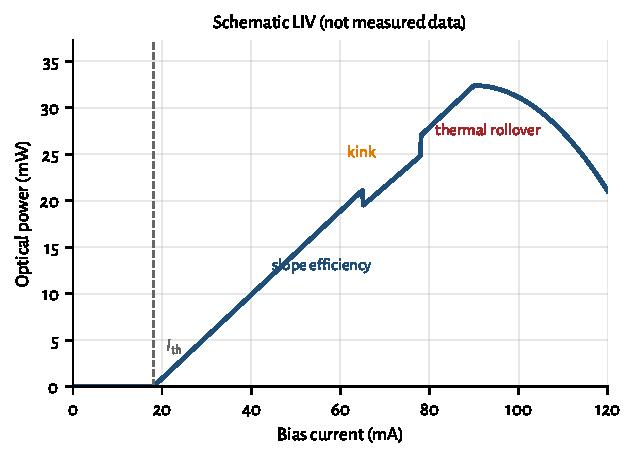
\includegraphics[width=0.85\linewidth]{figures/fig_liv_sketch.pdf}
\caption{Schematic LIV curve with threshold, slope, kink, and thermal rollover
labeled. Idealized for teaching; use measured LIV for pass/fail.
\label{fig:liv-sketch}}
\end{figure}

\paragraph{SMSR (side-mode suppression ratio).}
\firstterm{SMSR} SMSR is the power difference (dB) between the lasing mode and the
strongest side mode on an optical spectrum analyzer (OSA). Datacom single-mode
parts require high SMSR so side modes do not steal power or seed modal noise.
Spec-sheet floors are part-specific; treat the datasheet or ATP limit as
authoritative. SMSR collapse under temperature or aging is a reject: the laser is
leaving single-mode operation.

\paragraph{RIN (relative intensity noise).}
Measure RIN with a calibrated photodetector and RF spectrum analyzer (or a
dedicated RIN analyzer), under a controlled optical return loss. Distinguish
\emph{intrinsic} RIN (quiet bench, high ORL) from stressed
$\mathrm{RIN}_x\mathrm{OMA}$ used in Ethernet/MSA specs. IEEE 802.3 / 100G Lambda
class links cap $\mathrm{RIN}_{17.1}\mathrm{OMA}$ at $-136$~dB/Hz with 17.1~dB
ORL~\firstcite{rinspec}. Quiet datacom DFB/EML parts typically sit well below that
when feedback is controlled; CPO ELS designs care as much about feedback tolerance
as about the quiet number (\Cref{sec:rin-values,sec:rin}).

\begin{table*}[ht]
\refstepcounter{table}\label{tab:laser-meas}%
\centering
\setlength{\tabcolsep}{4pt}%
\footnotesize
\renewcommand{\arraystretch}{1.25}%
\begin{tabular}{@{}p{0.12\linewidth}p{0.18\linewidth}p{0.28\linewidth}p{0.36\linewidth}@{}}
\toprule
Parameter & Instrument & Pass/fail intent & Failure signature \\
\midrule
LIV & SMU + power meter / integrating sphere & $I_\mathrm{th}$, slope, kink-free bias window & high-temp rollover; kink in bias range \\
\addlinespace[1.5em]
SMSR & OSA & single-mode purity vs.\ datasheet/ATP & side modes rise with $T$ or age \\
\addlinespace[1.5em]
RIN & PD + ESA / RIN analyzer & intrinsic and stressed $\mathrm{RIN}_x\mathrm{OMA}$ & RIN rises with ORL; BER floor (\Cref{sec:rin}) \\
\addlinespace[1.5em]
Bias-driver noise & SMU vs.\ product bias board & $\mathrm{RIN}_{\mathrm{eq}}$ from $i_n$ (\Cref{sec:laser-drivers}) & RIN rises with rails on, flat vs.\ ORL \\
\addlinespace[1.5em]
Wavelength & OSA / wavemeter & grid placement, $d\lambda/dT$, $d\lambda/dI$ & walk off ring or MSA grid \\
\addlinespace[1.5em]
EAM bias (EML) & bias sweep + DCA/TDECQ & extinction, chirp, RLM & aging shifts absorption curve \\
\bottomrule
\end{tabular}
\par\medskip
{\raggedright\footnotesize\textbf{Table~\thetable.} Laser measurement playbook: what to
measure, with what, and what failure looks like.\par}
\end{table*}

Measure in order: LIV $\to$ SMSR $\to$ wavelength $\to$ RIN (quiet then
stressed ORL) $\to$ EAM or bias-driver checks as the path requires. Stop when
distributions across temperature and units support the bias window, grid, and
RIN policy in \Cref{tab:laser-prd} (see also
\Cref{tab:laser-engineering-checklist}). Do not keep measuring for its own
sake once those exits close.

\section{Laser drivers and the RIN budget}
\label{sec:laser-drivers}

Modulator RF drivers (\Cref{sec:drivers}) deliver swing and bandwidth into an EAM
or MZM. Laser \emph{bias} drivers are a different circuit: they set a quiet
constant current into the diode. Current noise on that path becomes optical
intensity noise and adds in the RIN budget of \Cref{sec:rin}. Confusing the two
is a common debug miss: a great SiGe PAM4 driver can still ruin a CW laser if its
supply or ground couples into the bias rail.

\paragraph{From current noise to equivalent RIN.}
Above threshold, optical power tracks bias approximately as
$P\propto(I-I_\mathrm{th})$. Relative intensity fluctuations then track relative
current fluctuations:
\[
\mathrm{RIN}_{\mathrm{eq,lin}}
\;\approx\;
\left(\frac{i_n}{I-I_\mathrm{th}}\right)^{\!2},
\qquad
\mathrm{RIN}_{\mathrm{eq}}[\mathrm{dB/Hz}]
\;=\;
20\log_{10}\!\left(\frac{i_n}{I-I_\mathrm{th}}\right),
\]
where $i_n$ is the one-sided current-noise density in A$/\sqrt{\mathrm{Hz}}$ at the
laser terminals (driver plus board pickup). The approximation assumes linear slope
efficiency and ignores intrinsic laser dynamics; it is a budget tool, not a device
model.

Worked numbers at $I-I_\mathrm{th}=50$~mA (typical CW DFB window): $i_n=500$~pA$/\sqrt{\mathrm{Hz}}$
maps to $\mathrm{RIN}_{\mathrm{eq}}\approx-160$~dB/Hz; $270$~pA$/\sqrt{\mathrm{Hz}}$
maps to about $-165$~dB/Hz. Commercial low-noise laser drivers quote roughly
$50$--$500$~pA$/\sqrt{\mathrm{Hz}}$ at 1~kHz depending on current range
(\Cref{tab:laser-driver-noise}); the Koheron DRV200 family is a concrete
example~\firstcite{koherondrv200}. Against a good datacom intrinsic RIN of
$-145$ to $-155$~dB/Hz (\Cref{sec:rin-values}), those 1~kHz densities look
comfortable. The budget tightens when $(I-I_\mathrm{th})$ is small (near
threshold, derated CW, or low-current VCSELs), when you integrate broadband
switching noise rather than a 1~kHz spot, or when SerDes/DSP rails dump discrete
tones onto the bias network.

\begin{table*}[ht]
\refstepcounter{table}\label{tab:laser-driver-noise}%
\centering
\setlength{\tabcolsep}{4pt}%
\footnotesize
\renewcommand{\arraystretch}{1.25}%
\begin{tabular}{@{}p{0.28\linewidth}p{0.18\linewidth}p{0.22\linewidth}p{0.26\linewidth}@{}}
\toprule
Driver class (example) & $i_n$ @ 1~kHz & $\mathrm{RIN}_{\mathrm{eq}}$ @ 50~mA & What it means \\
\midrule
Ultra-low-noise CW (DRV200-A-40) & 55~pA$/\sqrt{\mathrm{Hz}}$ & $\approx-179$~dB/Hz & Bench / metrology floor \\
\addlinespace[1.5em]
Low-noise CW (DRV200-A-200) & 270~pA$/\sqrt{\mathrm{Hz}}$ & $\approx-165$~dB/Hz & Typical quiet CW source \\
\addlinespace[1.5em]
Higher-current CW (DRV200-A-400) & 480~pA$/\sqrt{\mathrm{Hz}}$ & $\approx-160$~dB/Hz & Still below $-155$ intrinsic \\
\addlinespace[1.5em]
Shared digital LDO, poor PSRR & often $\gg$1~nA$/\sqrt{\mathrm{Hz}}$ + tones & can exceed $-145$ & False ``RIN'' on ESA \\
\bottomrule
\end{tabular}
\par\medskip
{\raggedright\footnotesize\textbf{Table~\thetable.} Bias-driver current noise converted to
equivalent RIN at $I-I_\mathrm{th}=50$~mA using
$\mathrm{RIN}_{\mathrm{eq}}=20\log_{10}(i_n/(I-I_\mathrm{th}))$. Densities for the
DRV200 rows are from the Koheron datasheet at 1~kHz; the last
row is qualitative (board-dependent).\par}
\end{table*}

\paragraph{CW / ELSFP / CW-WDM paths.}
For external CW sources feeding Si or TFLN modulators, design the bias path as a
low-noise current source with high supply rejection, local decoupling at the diode,
and a star ground that does not share return with SerDes switching currents.
Automatic power control (\firstterm{APC}) loops that close through a monitor PD
suppress slow drift; keep the loop bandwidth well below the RIN measurement band
and quiet enough that the loop itself does not inject intensity noise. ELSFP and
CW-WDM modules hide this circuitry inside the pluggable
(\Cref{sec:elsfp,sec:cwwdm-laser}); acceptance still needs module-level RIN with
the host bias and management rails connected, not only a quiet SMU on the bare die.

\paragraph{DML and EML.}
A \term{DML} shares one diode for bias and RF: a bias tee (or on-chip bias network)
combines a quiet DC source with the RF driver. Excess RF driver broadband noise,
poor tee isolation, or supply ripple on the bias arm all raise measured RIN and
chirp-related penalties. An \term{EML} splits the problem: keep the DFB bias as
quiet as a CW source, and treat the EAM RF driver under \Cref{sec:drivers}. EAM
drive amplitude sets extinction and chirp; DFB bias noise still lands in optical
intensity before the modulator.

\paragraph{What to measure on the bench.}
Bisect electrical vs.\ optical RIN:
\begin{enumerate}
\item Measure intrinsic RIN with a quiet SMU or known low-noise driver and high ORL
      (\Cref{sec:laser-params}).
\item Repeat with the product bias board / module rails connected. Any rise is
      driver or supply contribution, not laser physics.
\item Sweep ORL. Rise with reflection is feedback-driven laser RIN
      (\Cref{sec:rin-values}); rise independent of ORL points at the electrical path.
\item Look for discrete spurs on the ESA (switching frequencies, CMIS clocks). Spurs
      fail stressed $\mathrm{RIN}_x\mathrm{OMA}$ even when the broadband floor looks
      fine (\Cref{sec:rin-values}).
\end{enumerate}

\keyidea{Treat laser bias noise as a RIN term:
$\mathrm{RIN}_{\mathrm{eq}}\approx(i_n/(I-I_\mathrm{th}))^2$. Quiet CW drivers at
tens to hundreds of pA$/\sqrt{\mathrm{Hz}}$ usually sit under a $-145$~dB/Hz
intrinsic floor at 50~mA; digital supply pickup, near-threshold bias, and DML bias-tee
leakage are what actually burn the budget.}

\section{How lasers fail}
\label{sec:how-lasers-fail}

Six mechanisms account for most laser field returns. Each has a distinct
telemetry signature, so classify before you open FA.

\begin{description}
\item[Threshold current increase] $I_\mathrm{th}$ rises from its ship value at
      fixed temperature, usually with slope efficiency dropping in step. Points to
      active-region or facet degradation (\Cref{sec:laser-aging}).
\item[Slope efficiency degradation] Output power per unit bias current falls even
      when $I_\mathrm{th}$ is stable. A separate wear-out track from threshold rise;
      both show up on the same LIV sweep.
\item[Wavelength drift] The lasing line walks off its grid slot or ring resonance.
      Distinguish laser drift from TEC or ring drift by holding one actuator fixed
      and moving the other (\Cref{sec:locking-techniques,ch:wdm}).
\item[Aging (SMSR collapse, mode hopping)] Side modes grow relative to the main
      mode, or the laser hops between modes under temperature or current. An OSA
      trend over time is the tell.
\item[Thermal runaway] A positive feedback loop where higher junction temperature
      raises threshold current and cuts slope efficiency, so more drive power turns
      to heat for the same optical output, raising temperature further until the
      TEC saturates and the laser rolls over. Triggered by a failed or saturated
      TEC, a blocked heat path, or operation above the rated thermal class. Distinct
      from ordinary wear-out because it is fast (minutes, not months) once it
      starts; the failure-analysis handbook has the full symptom-to-cause
      breakdown (\Cref{sec:fm-thermal-runaway}).
\item[Monitor photodiode failure] The control loop's own sensor drifts or fails,
      so the laser looks unstable when the real fault is in the feedback path, not
      the gain medium (\Cref{sec:lasers-how-fails}).
\end{description}

\section{Separate thermal behavior from long-term aging}
\label{sec:laser-thermal-vs-aging}

Thermal response is reversible on the time scale of a temperature sweep or
cycle. It changes threshold current, slope efficiency, wavelength, EAM bias,
TEC current, and ring alignment. Measure it with controlled case-temperature
sweeps, loaded thermal corners, heater sweeps, and thermal cycling. Repeat the
measurement after returning to the starting temperature. Recovery points toward
an operating-point or control problem.

Long-term aging is cumulative. Threshold current rises, slope efficiency falls,
contacts degrade, defects grow, and an absorption or spectral curve can move
permanently. Measure those changes with HTOL, accelerated life testing, and
periodic LIV, spectrum, and modulation readouts. A temperature cycle can expose a
weak attach or calibration error, but it does not by itself establish a lifetime
acceleration model.

Do not merge the data sets. A high-temperature BER failure that clears at room
temperature needs thermal-margin work. A room-temperature baseline that keeps
moving after each stress interval needs an aging or damage hypothesis.

\section{Calibration: what drifts and what triggers retuning}
\label{sec:laser-calibration}

Calibration exists because no transmitter runs at a datasheet point. Every unit
has its own threshold, slope, absorption curve, quadrature point, and resonance,
and each of those moves with temperature and age. The operating points a product
actually stores are:

\begin{description}
\item[Laser bias / APC target] the bias current or monitor-PD power setpoint
      that holds launch power. Drifts as threshold rises and slope falls with
      age (\Cref{sec:laser-aging}); a drifting monitor PD corrupts it silently
      (\Cref{sec:lasers-how-fails}).
\item[EAM bias (EML)] the reverse-bias point that sets extinction and chirp.
      Moves with case temperature and with absorption-curve aging, so production
      parts store bias versus temperature, not one number.
\item[MZM quadrature] the phase bias that holds the modulator at its linear
      point. Drifts with temperature, stress, and age; a bias-control loop tracks
      it, and a railed loop is a telemetry alarm, not a retune request.
\item[Ring heater / lock point] the tuner power that aligns resonance to the
      laser line. Consumes headroom as ambient rises and neighbors heat; a railed
      DAC means the tuning range is exhausted
      (\Cref{sec:locking-techniques,sec:thermal-xtalk}).
\end{description}

Tables are usually segmented by temperature. Segment boundaries are a real
failure mode: the debug story in \Cref{sec:lasers-how-debugged} is a healthy
laser reading the wrong temperature segment after thermal cycling. Keep
calibration tables under change control and record the table version with every
test result, or failures cannot be replayed.

Recalibration should be triggered by evidence, not habit: a control-loop error
residual that no longer converges, an actuator (TEC, heater, bias DAC) that
approaches its rail, telemetry that disagrees with an external reference, a
temperature excursion beyond the table range, or a repair, rework, or firmware
change that invalidates stored coefficients. ATP must verify calibration at the
temperature corners the fleet will see, not only at the station ambient
(\Cref{sec:prod-corners}).

\section{How lasers are qualified}
\label{sec:how-lasers-qualified}

Qualification projects the failure mechanisms of \Cref{sec:how-lasers-fail}
forward from a short bench test to years of field life. Three stress classes do
the work:

\begin{description}
\item[HTOL (high-temperature operating life)] Run a sample lot at elevated
      temperature and bias for a fixed duration (often 1000 hours) and track LIV,
      SMSR, and wavelength drift. HTOL is the primary input to the Arrhenius life
      projection below.
\item[Burn-in] A shorter, sometimes 100\%-screen stress that removes
      infant-mortality units before ship, rather than projecting life. Burn-in
      trades test time for escape rate (\Cref{sec:hvm-test}).
\item[Environmental stress] Temperature cycling, damp heat, vibration, and shock
      catch packaging, attach, and mechanical failure modes that HTOL does not.
      They qualify different risks and should not be treated as substitutes for
      long-term aging data (\Cref{sec:gr468}).
\end{description}

Together with the Arrhenius acceleration factor, these three stresses turn a
qualification lot into a defensible FIT number.

\paragraph{Observable aging signatures.}
Watch LIV and spectrum over HTOL or field life:
\begin{itemize}
\item threshold rise and slope drop (active-region / facet degradation);
\item SMSR collapse (mode competition);
\item EAM bias creep on EMLs (absorption curve shift $\to$ TDECQ/RLM drift);
\item RIN rise under feedback (ORL or isolator failure);
\item COD\firstterm{COD} (catastrophic optical damage) at the facet under overstress.
\end{itemize}
Each signature should appear in the ATP and in field telemetry triage
(\Cref{sec:fleet-triage,sec:gr468}).

\section{Aging curves, derating, and fleet FIT}
\label{sec:laser-aging}

Lasers wear out. At fleet scale that is not a footnote; it sets architecture
(ELSFP vs.\ integrated laser) and operating policy (derating, burn-in).

\paragraph{Arrhenius life projection.}
\firstterm{Arrhenius} Telcordia GR-468-CORE qualifies optoelectronic parts with
accelerated stress (HTOL\firstterm{HTOL}, temperature cycle, damp heat) and projects field life
with Arrhenius acceleration~\firstcite{gr468}:
\[
\mathrm{AF}
= \exp\!\left[\frac{E_a}{k_B}\left(\frac{1}{T_\mathrm{use}}-\frac{1}{T_\mathrm{stress}}\right)\right],
\]
where $E_a$ is the activation energy for the wear-out mechanism under test, $k_B$
is Boltzmann's constant, and temperatures are absolute. Document $E_a$, sample
size, and confidence bounds when converting a 1000-hour HTOL lot into field-year
FIT. Activation energies are mechanism-specific; use the value justified in the
qual plan, not a generic number copied from another product.

\begin{figure*}[ht]
\centering
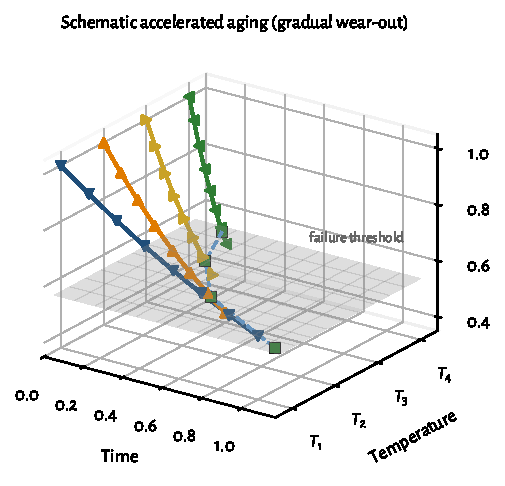
\includegraphics[width=0.92\linewidth]{figures/fig_accelerated_aging.pdf}
\caption{Schematic accelerated aging for gradual laser wear-out. A degradation
parameter (for example optical power at fixed bias, or threshold current rise
mapped to a falling health metric) is tracked versus time at several stress
temperatures $T_1 < T_2 < T_3 < T_4$. Higher temperature reaches the failure
threshold sooner. The dashed curve on the threshold plane is the
time-to-failure trend that Arrhenius acceleration turns into a use-condition
life estimate. Not measured data. Valid only for one thermally activated
mechanism with junction temperature as the stress variable; sudden modes such
as COD or ESD do not draw this surface.
\label{fig:accelerated-aging}}
\end{figure*}

\Cref{fig:accelerated-aging} is the mental model behind HTOL: same starting
health, faster drift at higher temperature, a defined end-of-life threshold, and
shorter time-to-failure as stress rises. For lasers the vertical axis is usually
tied to LIV or power at constant current; the temperature axis must be junction
temperature, not only chamber set point.

\paragraph{When the projection is valid.}
Acceleration assumes the stress speeds up the \emph{same} physical mechanism the
fleet will see. The projection fails in two ways: the stress activates a
mechanism the field never sees (solder creep or moisture ingress at a stress
temperature the product never reaches), or the field sees a mechanism the stress
never exercises (connector wear, bias-rail transients, thermal cycling from
traffic load). So a qual number is a hypothesis, not a fact: compare field-return
Pareto and failure signatures against the qual projection, and treat divergence
as evidence that $E_a$ or the mechanism model is wrong, not that the fleet is
unlucky (\Cref{sec:fleet-triage}). Sudden fails (COD, ESD, cracked fiber attach)
sit outside \Cref{fig:accelerated-aging}; classify those separately before you
fit Arrhenius parameters.

\paragraph{Derating.}
Run below absolute-max current, case temperature, and optical power. Derating
extends wear-out life and reduces COD risk. Uncooled datacom parts already sit near
thermal limits at high case temperature; cooled or faceplate ELSFP modules
(\Cref{sec:elsfp}) buy headroom by moving heat off the ASIC package.

\paragraph{Worked FIT example (assumptions labeled).}
\label{sec:fit-example}
FIT is failures per $10^9$ device-hours. For illustration only, assume 50~FIT per
laser (confirm against your supplier qual; do not treat 50 as a measured claim)
and a fabric with $5\times10^5$ lasers (order-of-magnitude for a large AI cluster
with several optical links per accelerator). Expected failures per day:
\[
\frac{5\times10^5 \times 50 \times 24}{10^9}
\approx 0.6\ \text{laser failures/day}.
\]
That is why field-replaceable ELSFP modules, burn-in screens, and derating are
design inputs, not afterthoughts (\Cref{ch:reliability}).

\section{ELS and ELSFP: architecture, pinout, qual}
\label{sec:elsfp}

\term{ELSFP}\firstterm{ELSFP} (External Laser Small Form-Factor Pluggable) is the
OIF form factor for faceplate-pluggable CW laser modules that feed co-packaged
optical engines~\firstcite{elsfp}. The lasers sit at the coolest part of the
system (front panel), hot-swap when they fail, and keep thermal load off the ASIC
and photonic engine.

\paragraph{Mechanical and optical.}
The module uses a card-edge electrical interface and a blind-mate multi-fiber
optical connector at the rear (MT-class ferrules), which improves eye safety for
high CW power by keeping live fiber inside the chassis~\firstcite{elsfp}. One ELSFP
can feed more than one optical engine. OIF defines optical power classes, thermal
classes, and wavelength assignments (e.g.\ DR-type 1311~nm and FR-type CWDM4
grids) so hosts and modules interoperate.

\paragraph{Management and hot-swap.}
ELSFP uses CMIS and the CMIS module state machine over TWI. On plug-in the module
resets, initializes management, and stays in low-power mode with lasers
\emph{off} until the host transitions it to ModuleReady and explicitly enables
lasers~\firstcite{elsfp}. \texttt{ModPrsL} and \texttt{IntL} support presence detect
and asynchronous alarms for safe hot-swap.

\paragraph{Electrical pinout (OIF-ELSFP-02.0 Table~7).}
Twenty-four contacts: multiple 3.3~V VCC and GND pins, module reset (\texttt{ResetL}),
low-power mode (\texttt{LPModeL}), two-wire serial management (\texttt{SCL}/\texttt{SDA}),
presence (\texttt{ModPrsL}), and interrupt (\texttt{IntL}), plus reserved pins for
future power/ground~\firstcite{elsfp}. \Cref{tab:elsfp-pins} summarizes the published
map.

\begin{table*}[ht]
\refstepcounter{table}\label{tab:elsfp-pins}%
\centering
\setlength{\tabcolsep}{4pt}%
\footnotesize
\renewcommand{\arraystretch}{1.25}%
\begin{tabular}{@{}p{0.08\linewidth}p{0.16\linewidth}p{0.28\linewidth}p{0.42\linewidth}@{}}
\toprule
Pin & Function & Requirements & Notes \\
\midrule
1--3 & VCC & 1.5~A, 3.3~V & with noise filtering \\
\addlinespace[1.5em]
4 & TBD & reserved & future power \\
\addlinespace[1.5em]
5 & ResetL & pull-up 10~k$\Omega$ & reset module, LVTTL \\
\addlinespace[1.5em]
6 & LPModeL & MMC on only & low-power mode (low), LVTTL \\
\addlinespace[1.5em]
7 & TBD & reserved & future ground \\
\addlinespace[1.5em]
8--10 & GND & 1.5~A, 3.3~V & with noise filtering \\
\addlinespace[1.5em]
11 & TBD & reserved & --- \\
\addlinespace[1.5em]
12 & SCL & TWI clock & host 4.7~k$\Omega$ pull-up; module $\ge$10~k$\Omega$ \\
\addlinespace[1.5em]
13 & SDA & TWI data & same pull-ups as SCL \\
\addlinespace[1.5em]
14 & TBD & reserved & --- \\
\addlinespace[1.5em]
15--17 & GND & 1.5~A, 3.3~V & with noise filtering \\
\addlinespace[1.5em]
18 & TBD & reserved & future ground \\
\addlinespace[1.5em]
19 & ModPrsL & shorted to GND in module & presence (low), LVTTL \\
\addlinespace[1.5em]
20 & IntL & pull-up 10~k$\Omega$ & interrupt, LVTTL \\
\addlinespace[1.5em]
21 & TBD & reserved & future power \\
\addlinespace[1.5em]
22--24 & VCC & 1.5~A, 3.3~V & with noise filtering \\
\bottomrule
\end{tabular}
\par\medskip
{\raggedright\footnotesize\textbf{Table~\thetable.} ELSFP electrical pinout
(adapted from OIF-ELSFP-02.0 Table~7). Lasers power only in ModuleReady after host
command; default on plug-in is lasers off~\firstcite{elsfp}.\par}
\end{table*}

\paragraph{Qual hooks for suppliers.}
Acceptance test plans should cover the checklist in \Cref{tab:atp-laser,sec:supplier-exec}:
laser LIV/SMSR/RIN inside the module; optical power-class compliance; connector
mating cycles and contamination/ORL; burn-in before ship; CMIS register sanity;
and thermal class at rated case temperature. Module bring-up must also prove the
CMIS enable sequence and ModuleReady laser policy (\Cref{sec:bringup}). Field
returns split between laser wear-out and connector/fiber-attach faults; keep both
in the triage tree (\Cref{sec:fleet-triage}).

\section{Optical safety and laser classes}
\label{sec:laser-safety}

\subsection{Hazard and laser classes}

Laser safety for interconnects is governed by IEC 60825-1 (laser product
classification) and IEC 60825-2 (optical-fiber communication systems,
OFCS)~\cite{iec60825}. Classes run from Class 1 (safe under normal use) through
Class 1M (safe unless the beam is collected by optics), Class 3R/3B, and Class 4.
At 1310~nm and 1550~nm the beam is invisible, which raises the operational risk:
technicians cannot see exposure. The retinal-hazard band ends near 1400~nm, but
corneal and skin hazards remain, and single-mode power confined to a $\sim$9~\textmu m
core is high radiance even at modest milliwatt levels.

Short-reach datacom modules are usually engineered so each fiber port stays Class 1
or Class 1M under rated launch power. That is a design constraint on EML/DFB bias
and on how much power each lane launches, not a label you add after the fact.

\subsection{Hazard level = aggregate, not per-lane}

The safety case scales with \emph{total} launched power at an accessible location,
not with a single DFB data sheet. CW-WDM and ELS banks concentrate many lines on one
MT or MPO ferrule (\Cref{sec:elsfp}). A connector that breaks out eight or sixteen
fibers can exceed a per-lane Class 1 budget even when each lane is modest. IEC
60825-2 assigns hazard levels (1 through 4) to each accessible port in the OFCS
based on the radiant power that could escape during service~\cite{iec60825}. That
is why ELS architecture and fiber count drive classification, not the laser chip
alone.

\subsection{Open-fiber protection: APR and ALS}

When fiber continuity is lost, open connectors and broken fiber can expose
hazardous power. \term{APR}\firstterm{APR} (automatic power reduction) holds
output at or below Hazard Level 1M and probes for re-mate with safe low-power
pulses. \term{ALS}\firstterm{ALS} (automatic laser shutdown) cuts power entirely
and was common on older SDH links; for modern high-power systems APR with
automatic restart is the preferred pattern because restart probes stay within the
hazard limit~\cite{g664}. ITU-T G.664 requires power reduction to Hazard Level 1M
within about 3~s of a continuity break, a restart inhibit window, and restart only
at safe power.

These mechanisms tie directly to CMIS and bring-up policy: lasers enable only when
the host commands ModuleReady (\Cref{sec:bringup,sec:cmis}). APR/ALS is what makes
a live ELSFP hot-swap survivable in a running rack (\Cref{sec:prod-corners}).

\subsection{What validation and ops owe}

Optical safety is a validation deliverable, not a compliance sticker. ATP should
verify APR/ALS trip threshold and timing on representative open-fiber faults; label
modules and cages with the rated class; document max launched power per port and per
MPO breakout; and write service procedures for multi-fiber connectors. At fleet
scale, a hot-swap runbook that assumes ALS works but was never tested in ATP is a
real hazard. Fold the APR/ALS check into the ELS hot-swap corner in
\Cref{sec:prod-corners} alongside mate-cycle and ORL tests.

\section{CW-WDM source validation}
\label{sec:cwwdm-laser}

Multi-wavelength CW sources (CW-WDM MSA) feed dense ring or filter banks on a PIC
(\Cref{sec:cwwdm,ch:wdm}). Validation is per-channel plus cross-channel:

\begin{itemize}
\item power flatness across $\lambda$ (uneven OMA after the modulator bank);
\item per-channel SMSR and wavelength grid placement;
\item channel crosstalk and residual ASE between lines;
\item lock to microring resonances under temperature and neighbor heating
      (\Cref{sec:locking-techniques,sec:thermal-xtalk,sec:siring});
\item RIN and ORL sensitivity for each line (\Cref{sec:laser-params,sec:rin-values}).
\end{itemize}

Examples: Ayar Labs SuperNova (CW-WDM MSA-compliant, feeds TeraPHY)
~\firstcite{ayar,cwwdm}; Broadcom ELSFP banks on Tomahawk CPO
(\Cref{sec:cpo-status,sec:elsfp}); quantum-dot comb lasers (Ranovus, Quintessent)
aimed at many $\lambda$ from one chip. Source tests live here; locking and on-chip
MUX live in \Cref{ch:wdm}.

\section{Light-source supply strategy}
\label{sec:laser-suppliers}

The sourcing decision follows the same architecture fork as the optical design:
buy a merchant source, buy a serviceable external module, or bind the source to
the photonic package. Evaluate each path by qualification ownership, second-source
portability, lot traceability, test access, field replacement, and change-control
rights. A vendor list ages quickly and does not answer those questions.

\begin{description}
\item[Merchant DFB, EML, or CW die] preserve module-level design freedom and can
      support a second source, but the integrator owns attach, driver match,
      screening, and package reliability.
\item[External CW-WDM or ELSFP module] moves source qualification and management
      into a replaceable unit. The system still owns connector, ORL, hot-swap,
      and host interoperability (\Cref{sec:elsfp,sec:cwwdm-laser}).
\item[Multi-wavelength source] reduces source count and can simplify WDM fan-out,
      but couples channel yield, power flatness, control, and replacement into one
      unit (\Cref{sec:cwwdm-laser}).
\item[Source integrated with the PIC] reduces optical interfaces and can improve
      density, but makes laser yield and wear-out part of package yield and
      service life.
\end{description}

\begin{table*}[ht]
\refstepcounter{table}\label{tab:laser-suppliers}%
\centering
\setlength{\tabcolsep}{5pt}%
\renewcommand{\arraystretch}{1.25}%
\begin{tabular}{@{}p{0.28\linewidth}p{0.68\linewidth}@{}}
\toprule
Approach & Qualification ownership and risk \\
\midrule
Merchant DFB/EML/CW die & Integrator owns attach, driver match, screen, and module qual \\
\addlinespace[1.5em]
External CW-WDM / ELSFP module & Supplier owns source module; system owns interface and service qual \\
\addlinespace[1.5em]
Multi-wavelength source & Shared yield, power-flatness, and replacement risk across channels \\
\addlinespace[1.5em]
Source integrated with PIC & Highest density; laser yield and life become package risks \\
\bottomrule
\end{tabular}
\par\medskip
{\raggedright\footnotesize\textbf{Table~\thetable.} Light-source sourcing paths
and the qualification ownership each one creates.\par}
\end{table*}
\FloatBarrier

\subsection{Reading the supplier ownership matrix}
\label{sec:laser-suppliers-read}

\Cref{tab:laser-suppliers} is a qualification-ownership map. The fork decides
who owns life data, screens, and field service, not only who ships a die.

\paragraph{Merchant DFB / EML / CW die.}

\textbf{Purpose.}
Who owns attach, driver match, module screen, and package reliability when
the source is a merchant die?

\textbf{Uncertainty removed.}
Die datasheets do not qualify the module. After ownership is explicit, the
integrator knows which FAIR, ATP, and HTOL packages stay in-house.

\textbf{Evidence the other party still owes.}
Die-level LIV, SMSR, RIN, and life sample data from the merchant; change
control on epi and process.

\textbf{Decision unlocked.}
Accept integrator-owned module qual, or reject the path if attach and screen
capability are missing.

\textbf{Risk if ownership is assumed wrong.}
You treat a die cert as module qual and discover attach or driver match in
the fleet.

\paragraph{External CW-WDM / ELSFP module.}

\textbf{Purpose.}
What does the source supplier own versus what the system still must qualify?

\textbf{Uncertainty removed.}
A replaceable ELS moves source life into a field unit, but connector, ORL,
hot-swap, and host interop remain system-owned (\Cref{sec:elsfp}).

\textbf{Evidence the other party still owes.}
Supplier: source-module ATP, CMIS, life, and mate ratings. System: optical
mate, ORL plant, service sequence, and engine bring-up with light present.

\textbf{Decision unlocked.}
Approve ELS architecture only when both ownership packs exist.

\textbf{Risk if ownership is assumed wrong.}
You qualify the laser module and skip the optical interface that fails first
in service.

\paragraph{Multi-wavelength source.}

\textbf{Purpose.}
How do channel yield, power flatness, and replacement couple across the
comb?

\textbf{Uncertainty removed.}
One weak channel can scrap or derate the whole source. Shared control means
shared field risk (\Cref{sec:cwwdm-laser}).

\textbf{Evidence required.}
Per-channel power and wavelength distributions, flatness over temperature,
and a replacement/service policy when one channel fails.

\textbf{Decision unlocked.}
Accept coupled yield, require channel redundancy, or split into multiple
sources.

\textbf{Risk if ownership is assumed wrong.}
You buy ``one laser'' economics and inherit N-channel fail modes without
N-channel screens.

\paragraph{Source integrated with PIC.}

\textbf{Purpose.}
When laser yield and wear-out become package risks, who owns life and
service?

\textbf{Uncertainty removed.}
Density gains remove a replaceable optical interface. Failures then pull the
engine or package, not a pluggable source.

\textbf{Evidence required.}
Package-level life, known-good attach, and a service model that matches
non-replaceable sources.

\textbf{Decision unlocked.}
Accept integrated risk for density, or keep ELS/merchant die for field
replaceability.

\textbf{Risk if ownership is assumed wrong.}
You qualify the die physics and underfund package yield and fleet
replacement cost.

\subsection{Why ownership order matters}

Choose the service and ownership model before you freeze the optical
architecture. An external source is replaceable and adds a managed interface.
An integrated source removes that interface and places source yield inside
the package. Qualify the architecture you will service, not only the laser
die.

\subsection{Learning summary}

\begin{description}
\item[Merchant die] Integrator owns module qual; merchant owns die life data.
\item[ELS / CW-WDM module] Supplier owns source; system owns mate, ORL, swap.
\item[Multi-wavelength] Channels share yield and replacement risk.
\item[Integrated PIC] Laser life is package life; plan service accordingly.
\end{description}

\aside{The fork is a reliability and ownership decision. An external source makes
the source replaceable but adds a managed optical interface. An integrated source
removes that interface but places source yield and wear-out inside the package.
Qualify the architecture you will service, not only the laser die.}

\section{Why lasers are the reliability bottleneck}

At the scale of a large optical fleet the laser is usually the
reliability-limiting component. It is an active device with wear-out physics that
passive optics and even photodiodes largely lack:

\begin{itemize}
\item \term{Catastrophic optical damage} (COD) at the facet.
\item Gradual facet and active-region degradation (accelerated by temperature,
      following Arrhenius kinetics; \Cref{sec:laser-aging}).
\item EAM aging in EMLs; coupling and solder drift in packaged assemblies.
\end{itemize}

Because failures scale with the number of lasers, a fleet of $100{,}000$+ links
turns a modest per-laser FIT rate into a steady stream of field failures
(\Cref{sec:fit-example,sec:gr468}). The mitigations shape architecture:
field-replaceable external laser sources (ELSFP, CW-WDM),
redundancy, burn-in screening to weed out infant mortality, and derating (running
lasers below their maximum to extend life).

\section{Margin erosion over temperature, lot, and life}
\label{sec:laser-margin-erosion}

A link rarely loses all margin in one event. The source can lose launch power as
slope efficiency falls. Connector loss and ORL can rise after service. EAM or
MZM bias can move. A ring can consume spectral headroom as its heater approaches
range. Driver noise can raise the BER floor while none of these changes violates
its stand-alone limit.

Track five ledgers:
\begin{description}
\item[Power margin] launch power, coupling, connector and MUX loss, receiver
      sensitivity, and aging reserve.
\item[Noise margin] intrinsic and feedback-driven RIN, bias-rail noise, receiver
      noise, and crosstalk.
\item[Timing margin] source and modulator bandwidth, dispersion, driver and host
      jitter, and equalization reserve.
\item[Spectral margin] laser wavelength, SMSR, filter or ring passband, thermal
      drift, and lock range.
\item[Control margin] headroom in APC, TEC, heaters, ring lock, bias DACs, and
      calibration tables. A railed loop can fail the link while the diode is
      still healthy.
\end{description}

Recompute the link at combined production corners. A nominal part at nominal
temperature says little about whether a slow loss in two ledgers will push a
tail unit across the pre-FEC BER limit. \Cref{sec:prod-corners,tab:fleet-triage}
carry the same ledgers into validation and fleet triage. The interview review
compresses this checklist in \Cref{sec:interview-margin-ledgers}. The wall-chart
form is \Cref{sec:tree-margin-budget}.

\begin{dectree}
Nominal system margin
  |
Temperature debit
  |
Voltage / power-quality debit
  |
Channel / connector debit
  |
Manufacturing variation
  |
Aging / wear
  |
Interoperability variation
  |
Remaining margin
  |
Above deployment requirement?
  |-- YES --> proceed
  |-- NO  --> redesign / restrict / recalibrate / reject
\end{dectree}

Not every debit is naturally in decibels. Depending on the subsystem, remaining
margin may be optical power, sensitivity, BER or FEC headroom, eye or TDECQ,
jitter, control range, lifetime, or yield. Validation often measures the net
externally visible result; do not double-count internal penalties the test
cannot separate (\Cref{sec:link-budget}).

\section{Engineering lens}
\label{sec:lasers-engineering-lens}

\subsection{How it works}

A laser is an active device with wear-out physics, which makes it both the first
line of the link budget and the fleet's reliability bottleneck. The chapter's
device families and LIV/SMSR/RIN measurements all serve one question: will this
source stay in spec for years at temperature?

\subsection{How it is measured}
\label{sec:lasers-how-measured}

Qualify the laser as a set of curves across temperature, bias, ORL, and age, not a
room-temperature data-sheet point. The measurement playbook (LIV, SMSR, RIN,
wavelength, and EAM checks with their instruments and pass/fail intent) is in
\Cref{sec:laser-params,tab:laser-meas}; the stress classes that project field life
are in \Cref{sec:how-lasers-qualified,sec:laser-aging,sec:gr468}~\cite{gr468}.

\subsection{How it fails}
\label{sec:lasers-how-fails}

The six field-return mechanisms are catalogued in \Cref{sec:how-lasers-fail}:
threshold rise, slope droop, wavelength drift, aging (SMSR collapse and mode
hopping), thermal runaway, and monitor-photodiode failure. Manufacturing adds die,
wafer, lot, and assembly spread to every one. The mechanism that most often
misleads triage is a healthy laser behind a bad feedback sensor, so it gets the
worked callout below.

\failuremode{Monitor photodiode drift}{Reported power falls or the bias loop moves,
but an external power meter does not show the same change.}{Monitor-PD responsivity
drift, transimpedance gain error, contamination in the monitor path, or a bad
calibration coefficient.}{External power meter, monitor current, bias current,
LIV, and loop error versus temperature.}{Repair the monitor path or calibration,
add disagreement alarms, and do not raise laser bias to compensate for a false
reading.}

\subsection{How it is debugged}
\label{sec:lasers-how-debugged}

For power degradation, compare external optical power, monitor current, bias, and
case temperature before changing the setpoint. Rerun LIV at the failing
temperature and compare it with ship data. If LIV moved, inspect SMSR, wavelength,
and RIN to classify active-region, facet, or modal change. If LIV is stable, move
to coupling, connector, monitor-PD, and control-loop checks. For a wavelength
excursion, inspect OSA data and TEC current together. For a bias anomaly, replace
the product driver with a quiet source before blaming the diode.

\debugstory{BER worsened after thermal cycling while average optical power stayed
in range.}{The DCA showed that extinction ratio had collapsed. LIV and SMSR were
unchanged, and an EAM bias sweep restored the eye.}{The light source was healthy,
but its modulator operating point was wrong.}{A calibration table used the wrong
temperature segment after the cycle.}{The table and screening limits were fixed,
and EAM bias sweep data became part of the thermal-cycle readout.}

\section{Engineering checklist}
\label{sec:lasers-checklist}

\begin{table*}[ht]
\refstepcounter{table}\label{tab:laser-engineering-checklist}%
\centering
\setlength{\tabcolsep}{4pt}%
\footnotesize
\renewcommand{\arraystretch}{1.25}%
\begin{tabular}{@{}p{0.20\linewidth}p{0.34\linewidth}p{0.40\linewidth}@{}}
\toprule
Decision or test & Question it answers & Evidence to retain \\
\midrule
Architecture & Does the source and modulation path close reach, rate, power, cost, and service? & Requirement allocation and rejected alternatives \\
\addlinespace[1.5em]
LIV & Is the operating window clear of threshold, kinks, and rollover? & Curves by unit, lot, temperature, and age \\
\addlinespace[1.5em]
Spectrum & Does wavelength and SMSR stay inside the assigned grid and filter passband? & OSA or wavemeter data across corners \\
\addlinespace[1.5em]
RIN and ORL & Does noise margin survive the reflection environment? & Quiet and stressed RIN with stated ORL and bandwidth \\
\addlinespace[1.5em]
Modulation & Does bias, drive, chirp, and bandwidth close the eye? & Bias sweeps, TDECQ or equivalent, and driver conditions \\
\addlinespace[1.5em]
Thermal behavior & Are reversible shifts within control and actuator range? & Temperature and heater sweeps, TEC current, recovery data \\
\addlinespace[1.5em]
Long-term aging & Which parameters drift permanently, and at what rate? & HTOL intervals, LIV, spectrum, and modulation trends \\
\addlinespace[1.5em]
Manufacturing & Can the ATP catch bad units and lot drift at useful test cost? & Limits, guard bands, GR\&R, yield, and reaction plan \\
\addlinespace[1.5em]
Fleet operation & Which monitors distinguish source, modulator, cooler, and optical path? & Telemetry map, alarm thresholds, and golden baselines \\
\bottomrule
\end{tabular}
\par\medskip
{\raggedright\footnotesize\textbf{Table~\thetable.} Source and modulation
engineering checklist. Each row ties a decision to evidence, not only a test
name.\par}
\end{table*}
\FloatBarrier

\subsection{Reading the laser engineering checklist}
\label{sec:lasers-checklist-read}

\Cref{tab:laser-engineering-checklist} is the decision sequence for a laser
program. Measurement methods for LIV, SMSR, RIN, and aging are taught earlier
in this chapter; the notes below focus on what each row unlocks and when you
may leave it.

\paragraph{Architecture.}

\textbf{Purpose.}
Does the source and modulation path close reach, rate, power, cost, and
service?

\textbf{Uncertainty removed.}
Component enthusiasm does not allocate requirements. After architecture you
have a chosen path, rejected alternatives, and owners for lock, attach, and
life (\Cref{tab:source-mod-matrix,tab:laser-suppliers}).

\textbf{Exit criteria.}
\textbf{Exit when} requirement allocation and rejected alternatives are
written and reviewed.

\textbf{Decision unlocked.}
Freeze the path into \Cref{tab:laser-prd}, or reopen the matrix.

\textbf{Risk if skipped.}
You validate a hero topology that cannot be serviced or powered in the rack.

\paragraph{LIV.}

\textbf{Purpose.}
Is the operating window clear of threshold, kinks, and rollover across unit,
lot, temperature, and age (\Cref{sec:laser-params})?

\textbf{Exit criteria.}
\textbf{Exit when} kink-free bias windows and distributions support the
bias policy.

\textbf{Decision unlocked.}
Set bias and derate, or reject lots / redesign the window.

\textbf{Risk if skipped.}
Soft BER and sudden dark fails appear without a ship baseline to compare.

\paragraph{Spectrum.}

\textbf{Purpose.}
Do wavelength and SMSR stay inside the assigned grid and filter passband?

\textbf{Exit criteria.}
\textbf{Exit when} OSA or wavemeter data across corners meet grid and SMSR
floors.

\textbf{Decision unlocked.}
Approve channel assignment, tighten temperature policy, or reject modal risk.

\textbf{Risk if skipped.}
WDM unlock and modal noise show up as ``random'' BER.

\paragraph{RIN and ORL.}

\textbf{Purpose.}
Does noise margin survive the reflection environment the plant will present
(\Cref{sec:rin-values})?

\textbf{Exit criteria.}
\textbf{Exit when} quiet and stressed RIN at stated ORL and bandwidth meet
the BER-floor budget.

\textbf{Decision unlocked.}
Approve isolator-free or isolator-required design; set plant cleaning rules.

\textbf{Risk if skipped.}
Lab RIN looks fine; field ORL raises the floor.

\paragraph{Modulation.}

\textbf{Purpose.}
Do bias, drive, chirp, and bandwidth close the eye at baud?

\textbf{Exit criteria.}
\textbf{Exit when} bias sweeps and TDECQ (or equivalent) at named driver
conditions meet Tx quality limits (\Cref{sec:tdecq}).

\textbf{Decision unlocked.}
Freeze EAM/MZM/ring bias policy, or reject the modulator class for this rate.

\textbf{Risk if skipped.}
Average power passes while the eye fails under temperature.

\paragraph{Thermal behavior.}

\textbf{Purpose.}
Are reversible shifts within control and actuator range?

\textbf{Exit criteria.}
\textbf{Exit when} temperature and heater sweeps, TEC current, and recovery
data show control headroom at loaded corners.

\textbf{Decision unlocked.}
Approve thermal envelope, add heaters/TEC margin, or derate case $T$.

\textbf{Risk if skipped.}
Lock and calibration faults are misread as permanent aging.

\paragraph{Long-term aging.}

\textbf{Purpose.}
Which parameters drift permanently, and at what rate
(\Cref{sec:laser-aging})?

\textbf{Exit criteria.}
\textbf{Exit when} HTOL intervals with LIV, spectrum, and modulation trends
support the life claim or force derate.

\textbf{Decision unlocked.}
Accept FIT/replacement plan, or hold ship for life risk.

\textbf{Risk if skipped.}
Useful-life planning uses hope instead of a mechanism.

\paragraph{Manufacturing.}

\textbf{Purpose.}
Can the ATP catch bad units and lot drift at useful test cost
(\Cref{tab:atp-laser})?

\textbf{Exit criteria.}
\textbf{Exit when} limits, guardbands, GR\&R, yield, and a reaction plan
exist for the ship screens.

\textbf{Decision unlocked.}
Open volume screens, or hold for process control.

\textbf{Risk if skipped.}
Qualified engineering lots diverge from production without a catch point.

\paragraph{Fleet operation.}

\textbf{Purpose.}
Which monitors distinguish source, modulator, cooler, and optical path
(\Cref{sec:fleet-triage})?

\textbf{Exit criteria.}
\textbf{Exit when} telemetry map, alarm thresholds, and golden baselines are
named and owned.

\textbf{Decision unlocked.}
Arm fleet triage; feed escapes back into ATP.

\textbf{Risk if skipped.}
Field tickets cannot separate laser wear from connector or TEC faults.

\subsection{Why the checklist order matters}

Architecture first, or you characterize the wrong path. LIV and spectrum
establish semiconductor and channel health before RIN and modulation argue
about floors and eyes. Thermal separates reversible control from permanent
drift before aging claims. Manufacturing and fleet close the loop so life and
screens stay honest after ship. Later rows must not compensate for a missing
architecture or ship baseline.

\subsection{Learning summary}

\begin{description}
\item[Architecture] Does the path close the product?
\item[LIV / spectrum / RIN] Is the source healthy in its plant?
\item[Modulation / thermal] Does the eye and control survive corners?
\item[Aging] What drifts permanently, and how fast?
\item[Manufacturing / fleet] Can you screen it and triage it at volume?
\end{description}

\section{Interview takeaway}
\label{sec:lasers-design-review}

\keyidea{Measure LIV, SMSR, wavelength, and RIN as distributions across
temperature, lot, and age. Tie each requirement to an ATP row, each life claim to
a physical mechanism, and each field alarm to a measurement that separates the
laser from its driver, monitor, cooler, and optical path.}

\paragraph{Three questions to test yourself.}
\begin{enumerate}
\item Why is the laser typically the reliability-limiting component in an optical
      link?
\item Optical power fell but the monitor photodiode reports no change. What do
      you check?
\item How would you qualify a second laser supplier without assuming the first
      supplier's failure distribution?
\end{enumerate}
